The GERDA (GERmanium Detector Array) experiment~\cite{Sch05} is designed to search for $0\nu\beta\beta$ decay of $^{76}$Ge. The main design feature is to operate naked germanium detectors directly in liquid argon in order to achieve extremely low background level. The concept is based on ideas presented in Ref~\cite{Heu95}. Detailed introduction of the experiment can be found in the first section of this chapter. GERDA is currently under construction in Hall A of the INFN Gran Sasso National Laboratory (LNGS), Italy. The current status of the experiment is described in the second section. The development of GERDA is divided into three phases. In the first phase (Phase I) unsegmented germanium detectors, which were previously used in IGEX~\cite{Aal02} and HdM~\cite{Hei04} experiments, will be re-deployed. The envisioned background level is $10^{-2}$~events/(kg$\cdot$keV$\cdot$year). In the second phase (Phase II) 18-fold segmented detectors, which currently are under construction, will be used in addition. The aimed background level is $10^{-3}$~events/(kg$\cdot$keV$\cdot$year). A later phase (Phase III) is under discussion in cooperation with the MAJORANA Collaboration~\cite{Gai03,Aal04} aiming at a one tonne scale experiment. The physics observation capabilities of three phases of GERDA are discussed in the last section.

\section{Concept}
\label{sec:gerda:conc}
The germanium detector has been used to detect ionizing radiation, particularly X-rays and $\gamma$-rays for years. It has energy resolution better than 1\% around the $Q$-value region of the $0\nu\beta\beta$ decay, which is among the bests in all $0\nu\beta\beta$ decay detectors introduced in Sec.~\ref{sec:gencon}. This provides very good separation of $0\nu\beta\beta$ decay signal from $2\nu\beta\beta$ decay background. However, the $Q$-value of the $0\nu\beta\beta$ decay of $^{76}$Ge, 2.039~MeV, is still lower than some of the natural radiation lines. Special designs are needed to reduce the background. Fig.~\ref{fig:gerda} shows the engineering drawing of the structure of GERDA. Each part of the structure is introduced in the following sections according to its functionality of reducing background from different sources.

\begin{figure}[tbhp]
  \centering
  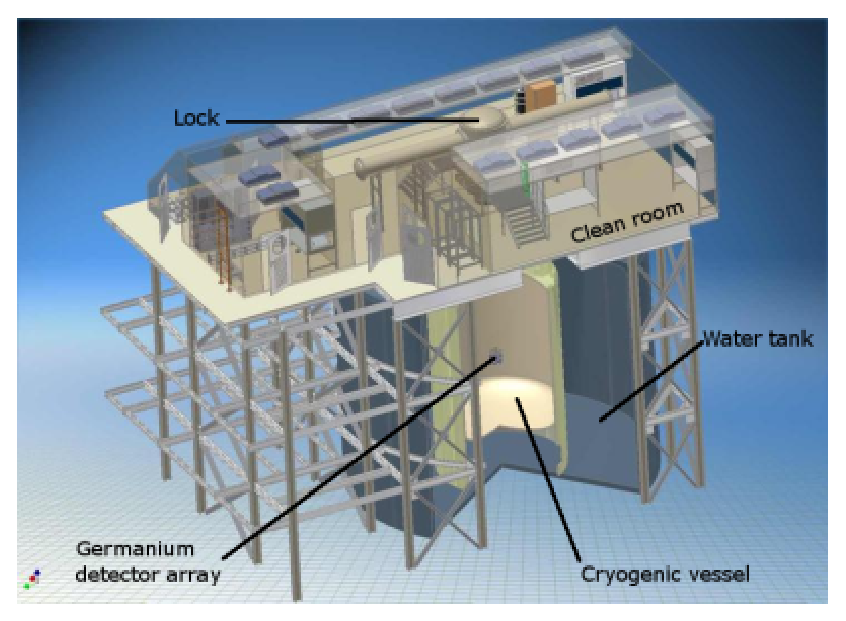
\includegraphics[width=0.7\textwidth]{gerda}  
  \caption{Structure of GERDA from engineer's view.}
  \label{fig:gerda}
\end{figure}

\subsection{Cosmic ray induced background}
\label{sec:gerda:loca}
In order to reduce the cosmic ray induced background GERDA was chosen to be located in Hall A of the INFN Gran Sasso National Laboratory (LNGS), Italy. LNGS is the largest underground facility in the world for low-background experiments. It can be accessed from a 10~km long highway tunnel under the Gran Sasso mountains. It has three experimental halls hosting a large variety of experiments, most of which focus on dark matter or neutrino physics. Fig.~\ref{fig:lngs} shows the location of GERDA in LNGS. The main experimental site of GERDA is between the Large Volume Detector (LVD) and a service tunnel across Hall A. The GERDA auxiliary and cryogenic storage system will be located in the service tunnel on the northeast side of Hall A.

\begin{figure}[tbhp]
  \centering
  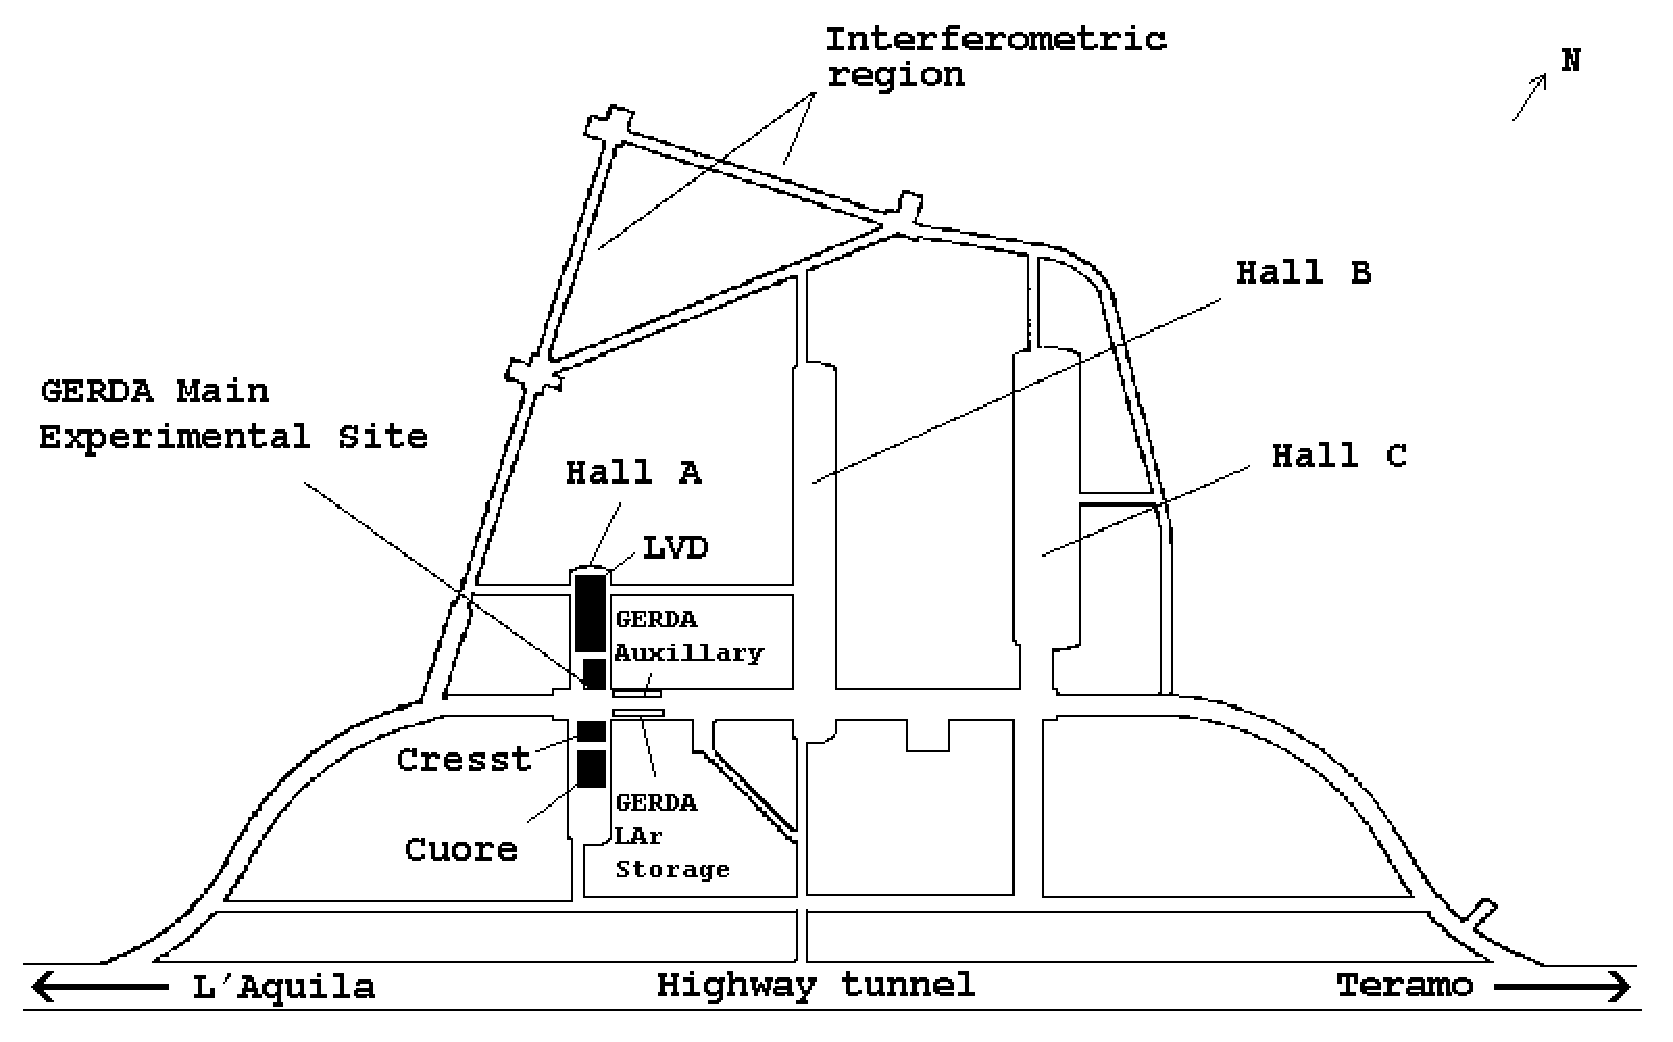
\includegraphics[width=0.8\textwidth]{lngs}  
  \caption{Location of GERDA in LNGS. The main experimental site of     GERDA is between the Large Volume Detector (LVD) and a service     tunnel across Hall A. The GERDA auxiliary and cryogenic storage     system will be located in the service tunnel on the northeast side     of Hall A.}
  \label{fig:lngs}
\end{figure}

The overburden of 1.4~km of rock on top of the experimental halls corresponds to 3.4~km meter of water equivalent (m.w.e). It reduces the cosmic ray induced muon flux by a factor of $10^{6}$, and neutron flux a factor of $10^{3}$ compared to the surface. The energy and angular distribution of cosmic ray muons in Hall A of LNGS have been precisely measured~\cite{Amb95, Lip91, Amb03}. A comprehensive study of cosmic ray induced muon and neutron background in underground laboratories can be found in Ref.~\cite{Mei06}.

In order to further reduce the muon induced background additional muon veto system will be implemented. Cosmic muons traversing the water buffer will cause Cherenkov radiation. To detect the radiation 66 photomultiplier tubes (PMTs) will be installed on the walls of the water tank. The positions of PMTs are optimized according to Monte Carlo simulation. Together with these PMTs the water tank could be operated as a Cherenkov detector. The detection efficiency is about 95\% depending on the incident angle of the muon. In order to compensate for the missing water volume around the neck of the cryostat plastic scintillator plates will be placed on top of the clean room. They are used to detect the muons entering the cryostat almost vertically. The combined detection efficiency is expected to be above 99\%.

\subsection{Background from rock}
\label{sec:gerda:rock}
To mediate and absorb the neutron radiation from the rock $\sim 630$~m$^{3}$ of ultra-pure water will be filled in a stainless steel tank with an outer diameter of 10~m and a height of about 8~m. Since liquid argon can be produced with a much greater purity than lead or even copper traditionally used for shielding, a total of approximately 98~t of liquid argon will be stored in a cryostat placed inside the water tank to shield $\gamma$-rays from the rock and water. The vessel is made of stainless steel with an internal copper liner. The height of the vessel is 5.88~m (7.62~m with the neck) while the outer diameter is 4.16~m.

\subsection{Background from detector suspension system and cables}
\label{sec:gerda:cable}
The detector array consists of hexagonally packed detectors with 3 layers. Up to 19 detectors can be placed per layer. The horizontal distance between the centers of two detectors is 9 cm. The vertical clearance between two detectors  is 5 cm. The array is divided into strings of vertically aligned detectors. Figure 3.3 (left) shows a seven string array of germanium detectors as designed for the Phase II of the GERDA experiment. The same figure (right) shows a top view of the full array indicat- ing the possible positions for the Phase I and Phase II detector strings as well as for the calibration sources.  The Phase I detectors are p-type diodes with a cylindrical closed-ended coaxial geom- etry. The detectors are enriched in 76Ge to a level of about 86\% and have masses between 0.9 kg and 2.9 kg.  The detectors for Phase II will be cylindrical true coaxial n-type diodes. The precise size of the detectors will depend on manufacturing details. The most likely dimensions are a height of 70 mm and a diameter of 75 mm. The detectors will be segmented. The segmentation scheme under consideration is a 6-fold segmentation in the azimuthal angle and a 3-fold segmentation in the height z. Light-weight holders were designed for the Phase II detectors together with a novel contacting scheme. The holders are made out of approximately 30 g of copper. Figure 3.4 (left) shows a Phase II prototype detector mock-up with its cabling and holder structure.  Figure 3.3: Left: An array of 7 × 5 germanium detectors as described in the text. Right: Top view of the full array indicating the possible positions for the Phase I and Phase II detector strings as well as for the calibration sources.

\begin{figure}[tbhp]
  \centering
  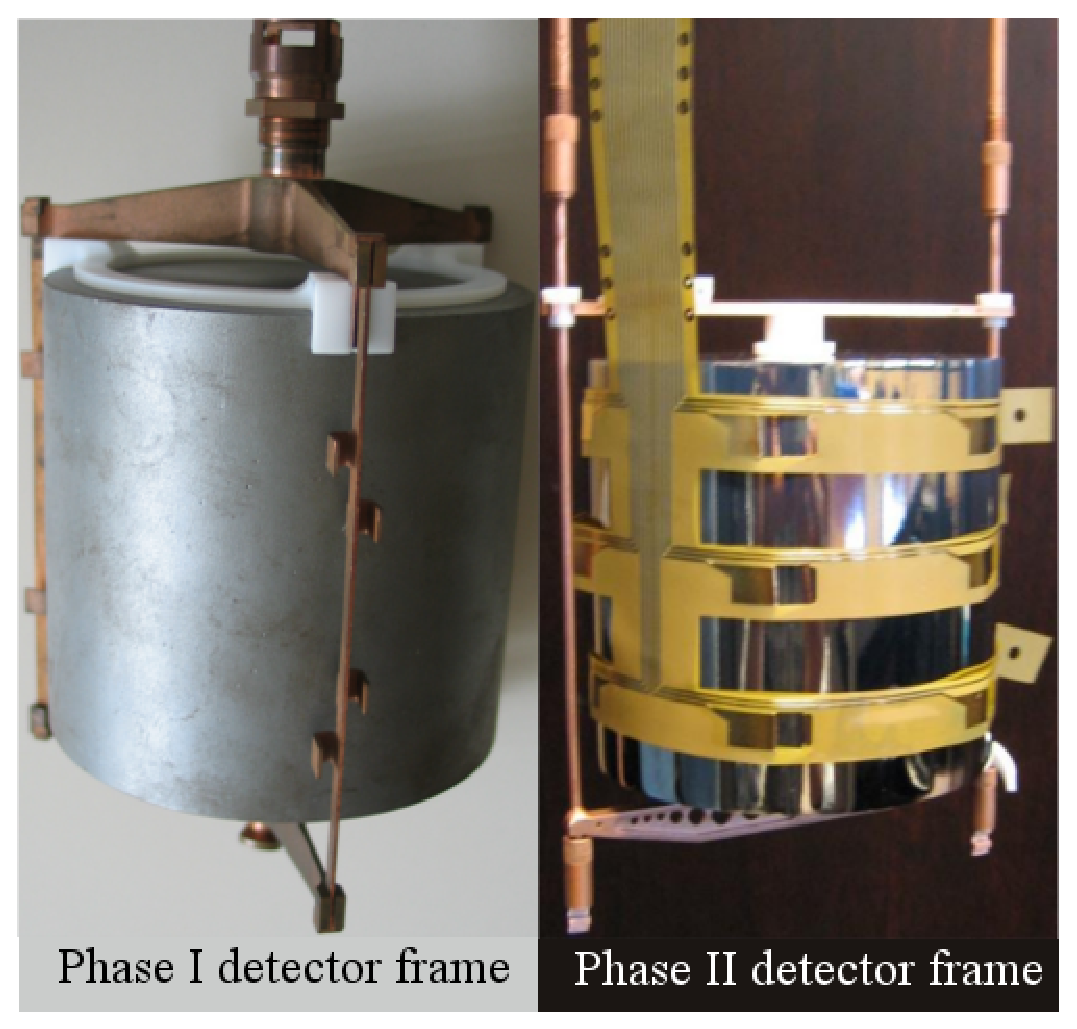
\includegraphics[width=0.33\textwidth]{detectorFrame}
  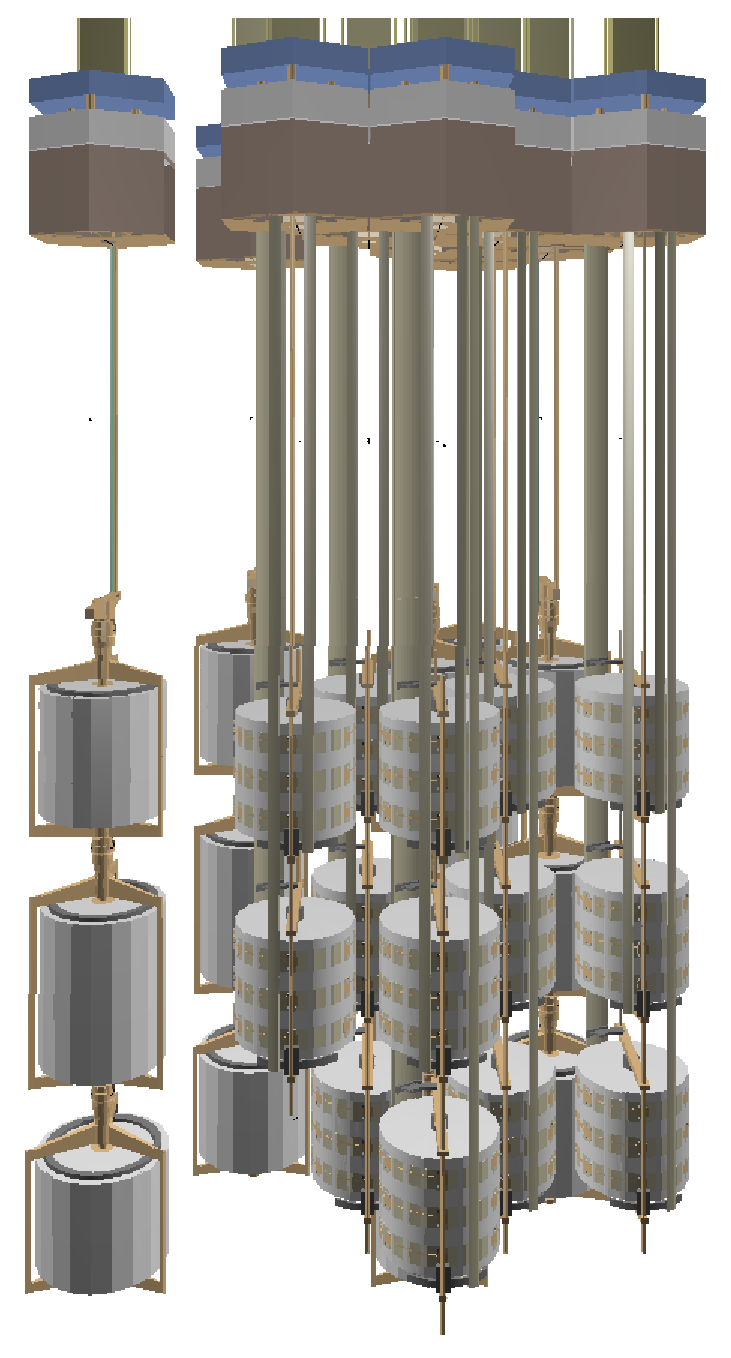
\includegraphics[width=0.2\textwidth]{array}
  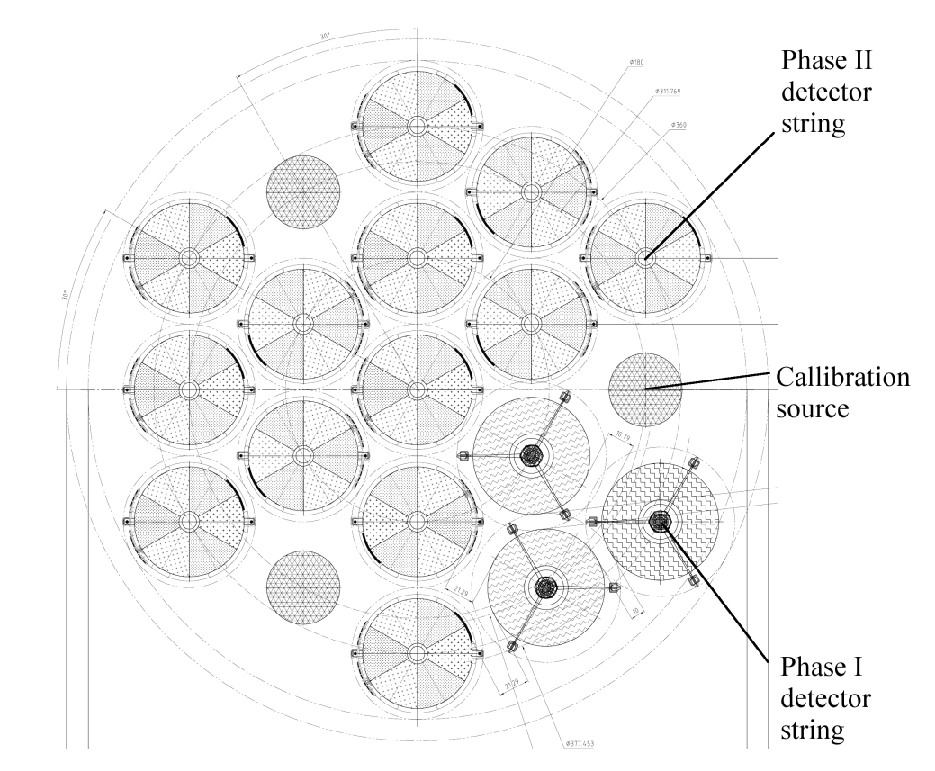
\includegraphics[width=0.45\textwidth]{arrayTop}
  \caption{Detector array configuration.}
  \label{fig:array}
\end{figure}


\section{Background from detector}
\label{sec:gerda:source}

\section{Time, detector, segment anti-coincidence}
\label{sec:gerda:anti}
\section{Pulse shape analysis}
\label{sec:gerda:psa}

\section{Liquid argon scintillator}
\label{sec:gerda:scin}

The natural abundance of $^{76}$Ge (7.6\%) is
not very high, hence additional enrichment is needed.

\section{Sensitivity}
\label{sec:gerda:sens}

The physics goal is to
confirm or disprove the observation claimed by part of the HdM
Collaboration. 

Assuming an exposure of
100~(kg$\cdot$year), an upper limit on $m_{\beta\beta}$ of
0.09-0.29~eV would be achievable. 

 The sensitivity of $m_{\beta\beta}$ would be down to
0.05~eV.

%%% Local Variables:
%%% mode:latex
%%% TeX-master: "thesis"
%%% End:
